\chapter{Vektorisasi Kata dan Dokumen}

\section{Teori}
\subsection{Vektorisasi}
Karena ketika menggunakan algoritma machine learning tidak bisa  secara langsung menggunakan teks melainkan teks tersebut harus diubah menjadi angka. Kita membutuhkan cara untuk merepresentasikan data teks untuk algoritma pembelajaran mesin, vektorirasi membantu mengubah teks biasa kedalam bentuk vektor yang dapat dimengerti oleh komputer atau machine learning. Kita mungkin ingin melakukan klasifikasi dokumen, sehingga setiap dokumen adalah "input" dan label kelas adalah "output" untuk algoritma prediksinyai. Algoritma mengambil vektor angka sebagai input, oleh karena itu kita perlu mengkonversi dokumen menjadi vektor angka dengan panjang tetap atau sama.
\par Untuk ilustrasinya misal,  saya memiliki kamus berisikan kata-kata {MonkeyLearn, is, not, great}, dan saya ingin membuat vektor teks "MonkeyLearn is great", saya akan memiliki vektor berikut: (1, 1, 0, 0, 1,) .

\subsection{Vektor Dataset Google}
Karena di dalam satu dataset berisikan setidaknya 3 Milyar kata dan kalimat. Yang dimana dimensi berisikan kata - kata unik dari data tersebut. Maka dari itu dimensi pada dataset Google bisa mencapai 300.

Untuk ilustrasinya, misalkan kita memiliki sebuah buku dengan tebal 1000 , dimana bukunya dibagi menjadi dua Chapter. Kemudian kita akan menggabungkan kata dari setiap Chapter tersebut. Maka akan didapatkan irisan yang akan berjumlah lebih dari 200. dikarenakan banyak kata yang berbeda beda.

\subsection{Konsep Vektorisasi Untuk Kata}
Konsepnya yaitu kata atau teks akan dihapuskan noisy datanya atau dihapus data yang tidak terpakai, seperti tag html jika ada, titik, koma, dll. Kemudian tokenization artinya kita akan mengelompokan kalimat menjadi token atua membagi kata kata menjadi potingan kecil. Baru setelah itu dilakukan normalisasi untuk mengubah datanya menjadi angka.

Ilustrasinya, misalnya ada beberapa kalimat seperti berikut :
\begin{itemize}
\item There used to be Iron Age.

Kemudian didapatkan token seperti berikut “There”,”was”,”to”,”be”,”used”,”Stone”,”Bronze,”Iron”,”Revolution”,”Digital”,”Age”,”of”,”Now”,”it”,”is”

Maka ketika di cek pada kalimat diatas hasilya seperti berikut 
\item There used to be iron age = [1,0,1,1,1,0,0,1,0,0,1,0,0,0,0]
\end{itemize}

\subsection{Konsep Vektorisasi Untuk Dokumen}
Hampir mirip dengan konsep kata, namun untuk di dokumen biasanya konsepnya digunakan untuk mencari kesamaan atau memprediksi seberapa sering menculan kata dalam 2 kalimat atau 2 paragraf.

Ilustrasinya, misalkan dalam sebuah artikel kita ingin mencari seberapa banyak kata "dimana" muncul. Maka dengan Doc2Vec dapat diprediksi hasilnya.

\subsection{Mean Dan Standar Deviasi}
\subsubsection{Pengertian}
Mean adalah nilai rata-rata dari beberapa buah data. Nilai mean dapat ditentukan dengan membagi jumlah data dengan banyaknya data.

Deviasi standar adalah ukuran ringkasan perbedaan setiap pengamatan dari rata-rata. Deviasi standar mengukur penyebaran data tentang nilai rata-rata. Ini berguna dalam membandingkan set data yang mungkin memiliki mean yang sama tetapi rentang yang berbeda.

\subsubsection{Contoh}
\begin{enumerate}
\item Misalkan kita sudah menghitung tinggi anjing.
\begin{figure}[ht]
\centering
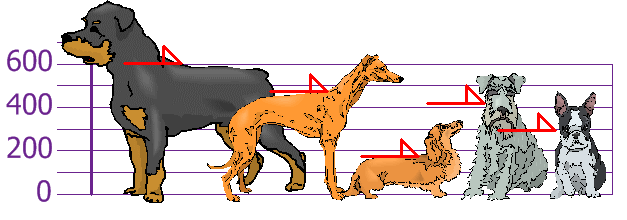
\includegraphics[scale=0.5]{figures/chapter5tasya1.png}
\caption{Contoh Mean dan Standar Deviasi }
\label{Teori}
\end{figure}
\item Tingginya dilihat dari bahu : 600mm, 470mm, 170mm, 430mm and 300mm.
\item Kita hitung mean atau rata ratanya, dengan menjumlahkan seluruh data dan membaginya dengan jumlah n nya hasilnya yaitu 394.
\item Kemudian kita ingin melihat berapa perbedaan tinggi dari anjing - anjing tersebut menggunakan variance. 
\item Baru Gunakan standar deviasi didapatkan hasil 147 mm . DEngan Deviasi Standar kita bisa tahau mana anjing dengan tinggi normal dan anjing yang kekurangan tinggi.
\begin{figure}[ht]
\centering
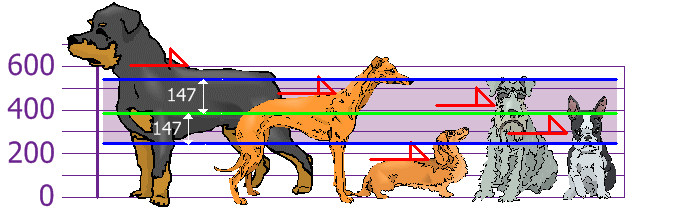
\includegraphics[scale=0.5]{figures/chapter5tasya2.png}
\caption{Contoh Mean dan Standar Deviasi }
\label{Teori}
\end{figure}

\subsection{Skip-gram}
Arsitektur model Skip-gram biasanya  mencoba untuk memprediksi kata konteks sumber (kata-kata sekitarnya) diberi kata target (kata tengah). Contohnya seperti berikut 
\begin{figure}[ht]
\centering
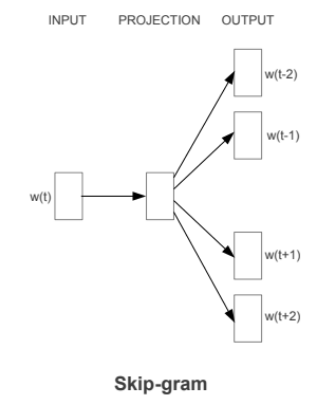
\includegraphics[scale=0.5]{figures/chapter5tasya3.png}
\caption{Contoh Skipgram }
\label{Teori}
\end{figure}
\end{enumerate}



\section{PRAKTEK PROGRAM}
\subsection{Mencoba Dataset}
\subsubsection{Vektor}
\begin{itemize}
\item Pada gambar diatas dapat dilihat bahwa vektor memiliki array sebanyak 300 dimensi. Untuk identitas sektor satu adalah 0.10
\begin{figure}[ht]
\centering
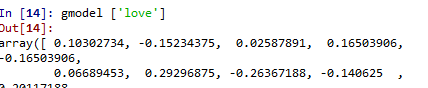
\includegraphics[scale=0.5]{figures/chapter5tasya4.png}
\caption{Vektor Love Tasya}
\label{Praktek}
\end{figure}


\item Pada gambar diatas untuk vektor faith dapat dilihat memliki nilai 0.26 , untuk similaritasnya cukup mendekati vektor love dimana faith dapat dikategorikan dalam satu kategori dengan love.
\begin{figure}[ht]
\centering
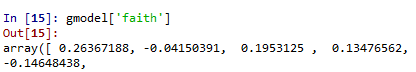
\includegraphics[scale=0.5]{figures/chapter5tasya5.png}
\caption{Vektor Faith Tasya}
\label{Praktek}
\end{figure}


\item Vektor fall hanya memiliki nilai minus yaitu -0.04 , dimana mesin memahami bahwa fall tidak terdapat dalam satu kategori yang sama dengan love dan faith
\begin{figure}[ht]
\centering
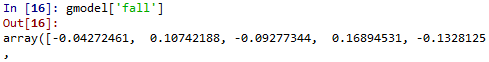
\includegraphics[scale=0.5]{figures/chapter5tasya6.png}
\caption{Vektor Fall Tasya}
\label{Praktek}
\end{figure}


\item  Vektor sick memiliki nilai identitas 1.82 dimana tidak mendekati love, faith maupun fall.
\begin{figure}[ht]
\centering
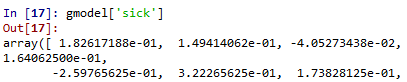
\includegraphics[scale=0.5]{figures/chapter5tasya7.png}
\caption{Vektor Sick Tasya}
\label{Praktek}
\end{figure}


\item Vektor clear memiliki nilai identitas -2,44 dan tidak mendekati nilai dari vektor fall sehingga tidak dapat dijadikan dalam satu kategori
\begin{figure}[ht]
\centering
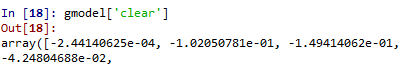
\includegraphics[scale=0.3]{figures/chapter5tasya8.png}
\caption{Vektor Clear Tasya}
\label{Praktek}
\end{figure}

\item Untuk vektor shine -0.12 tidak mendekati vektor manapun.
\begin{figure}[ht]
\centering
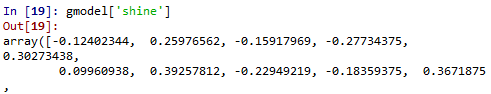
\includegraphics[scale=0.3]{figures/chapter5tasya9.png}
\caption{Vektor Shine Tasya}
\label{Praktek}
\end{figure}


\item Vektor bag memiliki i=nilai identitas -0.03 yang mendekati dengan vektor fall. SEhingga mesin memahami bahwa mungkin saja kedua vektor tersebut berada dalam satu kategori.
\begin{figure}[ht]
\centering
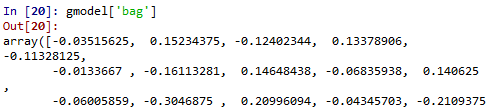
\includegraphics[scale=0.3]{figures/chapter5tasya10.png}
\caption{Vektor Bag Tasya}
\label{Praktek}
\end{figure}


\item Vektor car nilainya 0.13 mendekati vektor love dan faith sehingga mungkin dapat dikategorikan dalam satu kategori.
\begin{figure}[ht]
\centering
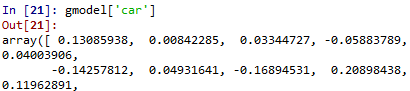
\includegraphics[scale=0.3]{figures/chapter5tasya11.png}
\caption{Vektor Car Tasya}
\label{Praktek}
\end{figure}


\item Vektor wash memiliki nilai 9.46 jauh dari vektor vektor lainnya.
\begin{figure}[ht]
\centering
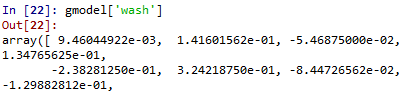
\includegraphics[scale=0.3]{figures/chapter5tasya12.png}
\caption{Vektor Wash Tasya}
\label{Praktek}
\end{figure}


\item Vektor motor memiliki nilai identitas 5.73 yang bisa mendekati vektor wash. Dapat dikatakan bahwa motor dapat dicuci jika diarti dalam satu kategori yang sama.
\begin{figure}[ht]
\centering
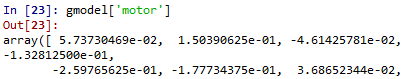
\includegraphics[scale=0.3]{figures/chapter5tasya13.png}
\caption{Vektor Motor Tasya}
\label{Praktek}
\end{figure}
\end{itemize}

\subsubsection{Similariti}
\begin{enumerate}
\item Lihat gambar berikut yang merupakan hasil prediksi similariti
\begin{figure}[ht]
\centering
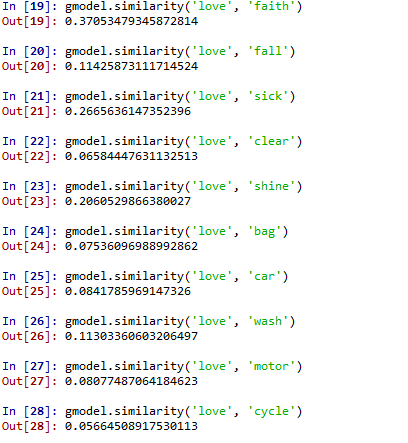
\includegraphics[scale=0.3]{figures/chapter5tasya17.png}
\caption{Similariti Tasya}
\label{Praktek}
\end{figure}

Dapat disimpulkan bahwa
\begin{itemize}
\item Untuk Love dan faith hasilnya adalah 37%
\item Untuk Love dan fall hasilnya adalah 11%
\item Untuk Love dan sick hasilnya adalah 26%
\item Untuk Love dan clear hasilnya adalah 6%
\item Untuk Love dan shine hasilnya adalah 20%
\item Artinya love dan faith memang dalam kategoruiyang sama misalnya dalam kategori percintaan. MEsin sudah mengetahui bahwa keduanya dapat dikategorikan sebagai percintaan.
\end{itemize}
\end{enumerate}

\subsection{Extract Words dan PermuteSentences}
\subsubsection{Extract Words}
ExtractWords merupakan function untuk menambahkan, menghilangkan atau menghapuskan, hal hal yang tidak penting atau tidakperlu di dalam teks. Dalam contoh dibawah ini. menggunakan function extract words untuk menghapus komen dengan python style , mencari data yang diinginkan, dan memberikan spasi pada teks.
\begin{figure}[ht]
\centering
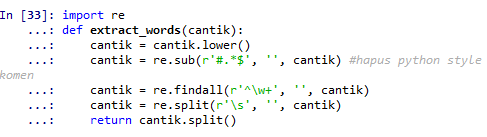
\includegraphics[scale=0.3]{figures/chapter5tasya15.png}
\caption{Extract Words Tasya}
\label{Praktek}
\end{figure}

\subsubsection{PermuteSentences}
PermuteSentences merupakan class yang digunakan unutm melakukan pengocokan secara acak pada data yang ada. Digunakan cara ini agar tidak terjadi kelebihan memori pada saat dijalankan. Contoh dibawah yaitu fungsi akan memanggil lenght. Yang kemudian mendefinisikan variabel req untuk lenght dam melakukan random choice yaitu pengocokan acak untuk kata car.
\begin{figure}[ht]
\centering
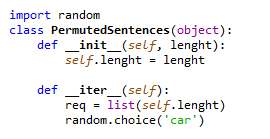
\includegraphics[scale=0.3]{figures/chapter5tasya16.png}
\caption{PermuteSentencesi Tasya}
\label{Praktek}
\end{figure}

\subsection{Fungsi Librari gensim TaggedDocument dan Doc2Vec}
Doc2vec adalah algoritma unsupervised untuk menghasilkan vektor untuk kalimat / paragraf / dokumen. Dan TaggedDocument merupaka function dari Doc2Vec untuk menampilkan tag kata atau kalimat yang diinginkan dari sebuah dokumen.

\begin{itemize}
\item Impor modul TaggedDocument dan modul Doc2Vec
\item Hasilnya seperti berikut
\begin{figure}[ht]
\centering
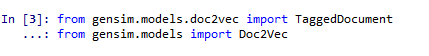
\includegraphics[scale=0.5]{figures/chapter5tasya18.png}
\caption{TaggedDocument Tasya }
\label{Praktek}
\end{figure}
\end{itemize}


\subsection{Menambahkan data Training Dari File Dengan Doc2Vec}
Yang harus dilakukan yaitu :
\begin{enumerate}
\item Import librari re atau request dari python dan import modul os untuk memungkinkan kita menggunakan operasi sistem sesuai yang dibutuhkan.
\item Medefinisikan variabel unsup sentences yang berisikan variabel kosong.
\item Panggil data training dan data testing dari file yang telah disediakan
\item Kemudian coba data tersebut
\end{enumerate}

Untuk lebih jelasnya, berikut hasil percobaan dari praktek yang dilakukan
\begin{verbatim}
for dirname in ["/train/pos", "/train/neg", "/train/unsup", "/test/pos", "/test/neg"]:
    for fname in sorted (os.listdir("aclImdb/"+dirname)):
        if fname[-4:] == '.txt':
            with open("aclImdb/"+dirname+"/"+ fname, encoding = 'UTF-8') as f:
                sent = f.read()
                words = extract_words(sent)
                unsup_sentences.append(TaggedDocument(words,[dirname+"/"+fname]))
\end{verbatim}
\begin{itemize}
\item Untuk skrip diatas mengambil contoh dataset dari Imdb yang kemudian memanggil data training dan data testing nya.
\item File tersebut diambil dari folder aclImdb
\item File yang dibuka berbentuk teks atau berekstensi txt
\item Kemudian file yang dibuka tadi diasiasikan sebagai f
\item variabel sent akan membaca f
\item Variabel words akan memanggil dan mengirimkan fungsi extract words dari skrip sebelumnya
\item KEmudian list dari unsup sentences akan diupdate dengan menambahkan objek baru dan diberi tag. berikut hasilnya
\begin{figure}[ht]
\centering
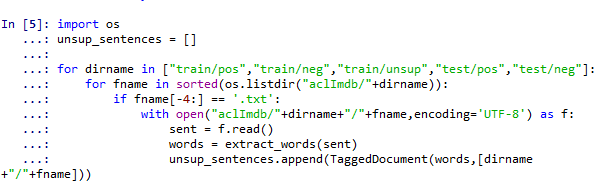
\includegraphics[scale=0.5]{figures/chapter5tasya20.png}
\caption{Data Training Imdb Tasya}
\label{Praktek}
\end{figure}
\end{itemize}
\begin{itemize}
\item Untuk contoh dibawah pun sama seperti ynag diatas, bedanya hanya untuk contoh kedua ini dilakukan proses token dan datasetnya dari review polarity.
\begin{figure}[ht]
\centering
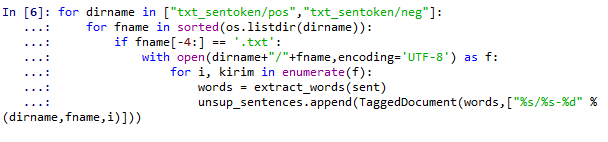
\includegraphics[scale=0.5]{figures/chapter5tasya21.png}
\caption{Data Training Polarity Tasya}
\label{Praktek}
\end{figure}

\item Untuk contoh dibawah pun sama seperti yang diatas, bedanya hanya untuk contoh kedua ini dilakukan proses token dan datasetnya dari review rotten tomatoes.
\begin{figure}[ht]
\centering
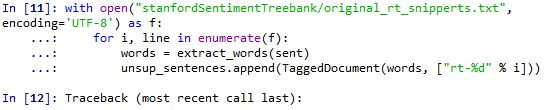
\includegraphics[scale=0.5]{figures/chapter5tasya22.jpg}
\caption{Data Training Tomatoes}
\label{Praktek}
\end{figure}
\end{itemize}

\subsection{Mengapa Harus Dilakukan Pengocokan Dan Pembersihan Data}
Pengocokan dilakukan untuk mendapatkan hasil yang lebih akurat pada saat melakukan score, karena pengocokan mempengaruhi performa positif negatifnya dari scoring.

Kemudian Pembersihan data dilakukan untuk membersihkan tag spasi ataupun data noisy yang tidak diperlukan dalam dokumen.
\begin{itemize}
\item Import dulu librari re atau request
\item Kemudian Disini akan mendefinisikan function extract words untuk menghapus tag html, hapus tanda petik dan lainnya
\item Setelah itu Data akan dirandomatau dilakukan pengocokan dengan mengimport librari modul dengan mendefinisikan class PermuteSentences. BErikut skrip lengkapnya
\item \begin{verbatim}
import re
def extract_words(sent):
    sent = sent.lower()
    sent = re.sub(r'<[^>]+>', ' ', sent) #hapus tag html
    sent = re.sub(r'(\w)\'(\w)', ' ', sent) #hapus petik satu
    sent = re.sub(r'\W', ' ', sent) #hapus tanda baca
    sent = re.sub(r'\s+', ' ', sent) #hapus spasi yang berurutan
    return sent.split()

import random
class PermuteSentences(object):
    def __init__(self, sents):
        self.sents=sents
        
    def __iter__(self):
        shuffled = list(self.sents)
        random.shuffle(shuffled)
        for sent in shuffled:
            yield sent
\end{verbatim}
\item Berikut merupakan hasil dari pengocokan dan pembersihan data
\begin{figure}[ht]
\centering
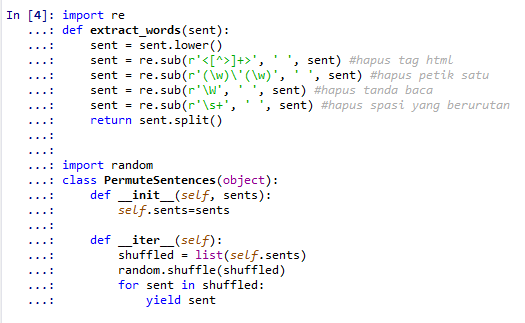
\includegraphics[scale=0.5]{figures/chapter5tasya19.png}
\caption{Pengcokan Dan Pembersihan Data Tasya}
\label{Praktek}
\end{figure}
\end{itemize}

\subsection{Mengapa Model Harus Di Save Dan Temporari Training Harus Dihapus}
\begin{itemize}
\item Sebelum model di save atau disipman lakukan pengocokan terlebih dahulu seperti berikut.
\begin{figure}[ht]
\centering
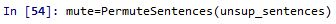
\includegraphics[scale=0.5]{figures/chapter5tasya23.jpg}
\caption{Save Model Tasya}
\label{Praktek}
\end{figure}
\item Kemudian setelah itu gunakan perintah Doc2Vec load dan memasukan nama file setelah disimpan.
\begin{figure}[ht]
\centering
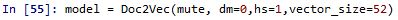
\includegraphics[scale=0.5]{figures/chapter5tasya24.jpg}
\caption{Save Model Tasya}
\label{Praktek}
\end{figure}
\item Ketika model telah di save, barulah hapus temporari dengan skrip berikut. Maka hasil dari kedua praktek diatas adalah sebagi berikut
\begin{figure}[ht]
\centering
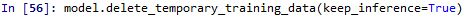
\includegraphics[scale=0.5]{figures/chapter5tasya25.jpg}
\caption{Save Model HAsil Tasya}
\label{Praktek}
\end{figure}
\begin{figure}[ht]
\centering
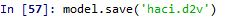
\includegraphics[scale=0.5]{figures/chapter5tasya26.jpg}
\caption{Save Model  HasilTasya}
\label{Praktek}
\end{figure}

Hal yang dapat disimpulkan yaitu :
Model disave untuk memudahkan kita dalam meng-edit file, kita tidak perlu mengetik ulang semua skrip dan tinggal membuka file tersebut jika ingin menguji ulang modelnya.
Temporari training merupakan data training yang sebelumnya kita gunakan untuk mencoba skripnya, namun karena kita telah membuat modelnya dan untuk menghemat memori dilakukan penghapusan temporari training agar tidak terjadi lag ataupun hal lainnya.
\end{itemize}


\subsection{Infer Code}
Infer vektor digunakan untuk mengkalkulasikan berapa vektor dari kata yang dberikan. Atau dengan kata lain mengubah kata yang diberikan menjadi bentuk vektor. Dari model yang telah dibuat
\begin{itemize}
\item Masukan skrip berikut yang artinya akan memanggil infer vector untuk mengkompres kalimat berikut menjadi bentuk vektor
\begin{verbatim}
model.infer_vector(extract_words("I will go home"))
\end{verbatim}
\item Hasilnya seperti berikut
\begin{figure}[ht]
\centering
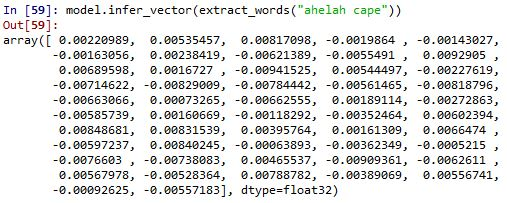
\includegraphics[scale=0.5]{figures/chapter5tasya32.jpg}
\caption{Infer Code Tasya}
\label{Praktek}
\end{figure}
\end{itemize}

\subsection{Cosine Similarity}
Cosine similarity digunakan untuk melihat kesamaan atau kemiripan dari suatu kalimat/paragraf yang diinginkan. Apakah kalimat tersebut dapat dikategorikan dalam satu kategori atau tidak.
Disini saya akan membandingkan beberapa kalimat seperti berikut :
\begin{itemize}
\item Masukan perintah berikut diamana sistem akan mengimpor cosine similarity dan kemudian gunakan function infer vector untuk membandingkan dua kalimat berikut.
\item Hasilnya seperti berikut, data dilihat bahwa kata 
\begin{verbatim}
from sklearn.metrics.pairwise import cosine_similarity
cosine_similarity(
        [model.infer_vector(extract_words("she going to school, after wash hand"))],
        [model.infer_vector(extract_words("Services sucks."))])
\end{verbatim}
\begin{figure}[ht]
\centering
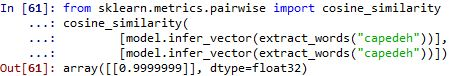
\includegraphics[scale=0.5]{figures/chapter5tasya27.jpg}
\caption{Infer Code Tasya}
\label{Praktek}
\end{figure}
\end{itemize}

\subsection{Score Dari Cross Validation}
\begin{itemize}
\item Pertama kita akan mengimpor KNN RF dan numpy
\begin{verbatim}
from sklearn.neighbors import KNeighborsClassifier
from sklearn.ensemble import RandomForestClassifier
from sklearn.model_selection import cross_val_score
import numpy as np
\end{verbatim}
\item Kemudian lakukan cek score dengan perintah berikut 
\begin{verbatim}

scores = cross_val_score(clf, sentvecs, sentiments, cv=5)
np.mean(scores), np.std(scores)
\end{verbatim}

\item Hasilnya seprti berikut
\begin{figure}[ht]
\centering
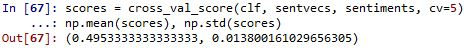
\includegraphics[scale=0.5]{figures/chapter5tasya29.jpg}
\caption{Score Cross Validation Tasya}
\label{Praktek}
\end{figure}
\end{itemize}

\subsection{Penanganan Error}
\subsubsection{Error MEmory}
\begin{enumerate}
	\item
Berikut ini merupakan eror yang didapatkan saat menjalankan program diatas
\begin{figure}[ht]
\centering
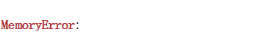
\includegraphics[scale=0.5]{figures/chapter5tasya31.jpg}
\caption{Error Memory Tasya }
\label{Error}
\end{figure}
\item Eror diatas merupakan memori eror dimana memori dari ram hampir terpakai semua sehingga program tidak dapat dijalankan. Cara mengatasinya yaitu
\begin{itemize}
\item Membatasi penggunaan memori
\item Menambah kapasitas ram
\item Jika terjadi blank screen atau lag, force shutdown. Dan jangan membuka aplikasi yang memakan banyak memori lainnya.
\end{itemize}
\end{enumerate}

